%!TEX root = ./icml2016.tex

\section{Related Work}

The literature on data factorisation or low-rank approximation is vast. 
We give a brief overview of related work with respect to three
orthogonal dimensions, a statistical method, learning strategy, and 
representation of data, which are helpful to formulate our problem.
We review important perspectives within each dimension below:
\begin{description}
\item[Statistical method] With an statistical assumption used to develop 
underlying model structure, we broadly categorise models into Bayesian 
and non-Bayesian models?.
\item[Learning strategy] The models passively learn from labels of given 
data points, or the models actively learn by  requesting data points 
to be labeled.
\item[Data representation] Data for a factorisation problem can be 
represented as a matrix or tensor. A graph representation of tensor reveals
a compositional structure of the data.
\end{description}
In Table \ref{tbl:relatedwork}, we summarise the previous work based on 
the combination of the different perspectives of each dimension.

The knowledge base construction has been widely focused in the natural 
language processing communities. Manual data acquisition with human crafted 
or automatically inferred synthetic rules or distant supervision on a large
amount of unlabeled text are the main tools to construct \cite{fader2011identifying,Mintz2009}.
Recently, \citet{kajino2015active} show active knowledge base construction
algorithm based on the low-rank structure. They proposed active 
multi-relational data construction (AMDC) with two separate problems: 
a knowledge base population and predictive model construction, and show 
that these two goals cannot be achieved at the same time. In this work, 
we show that it can be achieved at the same time with a properly designed
exploration and exploitation scheme that has been shown in the matrix 
factorisation problem \cite{kawale2015efficient}.

% Compositional relation learning \cite{Neelakantan2015}

\begin{table}[t]
\centering
\caption{\label{tbl:relatedwork}The categorisation of factorisation problems with respect to the three orthogonal dimensions. The capital letters indicate Bayesian(B)/Non-Bayesian(N) method, Passive(P)/Active(A) learning, and Matrix(M)/Tensor(T)/Compositional(C) structure. In this work, we tackle the problems denoted by *.}
\vskip 0.15in
\begin{tabular}{c c c l}
B/N & P/A & M/T/C & References	\\ \hline \hline

N & P & M & \citet{lee1999learning}\\ \hline

\multirow{2}{*}{N} & \multirow{2}{*}{P} & \multirow{2}{*}{T}& \citet{nickel2011three}\\
& & & \citet{kolda2009tensor}\\ \hline

N & P & C & \citet{Neelakantan2015} \\ \hline

N & A & M & \citet{ruchansky2015matrix}\\  \hline

N & A & T & \citet{kajino2015active} \\  \hline

%N & A & C & \\  \hline

B & P & M & \citet{mnih2007probabilistic}\\ \hline

\multirow{2}{*}{B} & \multirow{2}{*}{A} & \multirow{2}{*}{M}&  \citet{kawale2015efficient} \\
& & & \citet{sutherland2013active}\\ \hline

\multirow{2}{*}{B} & \multirow{2}{*}{P} & \multirow{2}{*}{T}& *, \citet{xiong2010temporal}\\
& & & \citet{schmidt2009probabilistic} \\ \hline

B & A & T & * \\ \hline

B & P & C & * \\ 

%B & A & C & Future work \\ 
\end{tabular}
\end{table}

%\begin{itemize}
%\item [B,A,M] Efficient Thompson Sampling for OnlineMatrix-Factorization Recommendation\cite{kawale2015efficient}. Active learning and search on low-rank matrices \cite{sutherland2013active}. Collaborative filtering as multi armed bandit \cite{guillou2015collaborative}
%\item [N,A,M] Matrix completion with queries \cite{ruchansky2015matrix}.
%\item [B,P,M] PMF \cite{mnih2007probabilistic} ...
%\item [N,P,M] NMF\cite{lee1999learning} ...
%\item [B,P,T] Bayesian Tensor Factorisation models. CANDECOMP/PARAFAC (CP) decomposition \cite{xiong2010temporal,schmidt2009probabilistic}, CP and TUCKER3 \cite{yilmaz2012algorithms}
%\item [N,A,T] Populating knowledge graph with active learning (IBM) \cite{kajino2015active}
%\item [N,P,T] Rescal \cite{nickel2011three}, TransE \cite{bordes2013translating}, and many others.
%\item [N,P,C] Compositional vector space model \cite{Neelakantan2015}, 
%\end{itemize}
%
%Might be relevant, but not positioned in the figure.
%\begin{itemize}
%\item Clustering based Bayesian approach for learning relations: Infinite relational model based on entity clustering \cite{kemp2006learning}.
%\item Path ranking algorithm (graph feature model) \cite{Lao2010}
%\end{itemize}

%\begin{figure}[t]
%	\centering
%	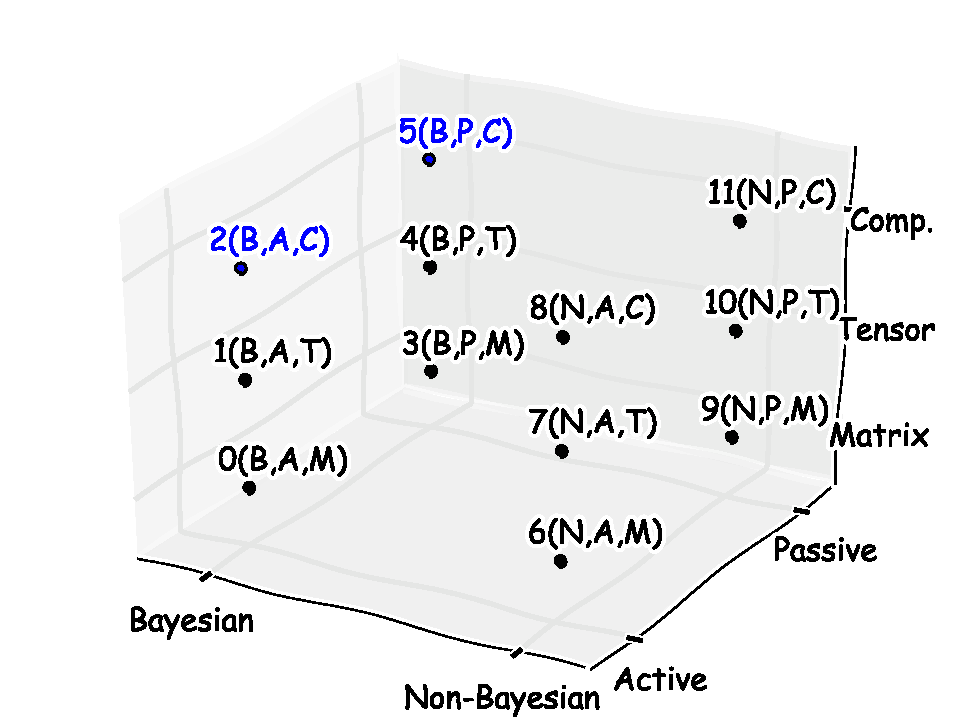
\includegraphics[width=\linewidth]{images/3d_plot.pdf}			
%	\caption{\label{fig:related3d}Scope of our work}
%\end{figure}
